% Section content template for individual Educative lessons
% This file contains the actual content for a specific section
% Generated from Educative API section content

% Section: Getting Ready: Movie Ticket Booking System
% Section ID: 6553143930519552
% Section Slug: getting-ready-movie-ticket-booking-system
% Generated: 2025-12-12T14:17:42.061242

\subsection{Problem definition}\label{DFpOXaHfjUJHQ4h6AROJx-1}
\\
The \textbf{movie ticket booking system} enables customers to search for movies, browse showtimes across various cinemas in multiple cities, select preferred seats, and securely book tickets online. The system manages comprehensive information about cinemas, locations, cinema halls, movie listings, and scheduled shows. Customers can view a live seating layout for each show, select and reserve available seats, receive booking confirmations, and complete payment.
\\
In this LLD interview case study, you'll focus on:

\begin{itemize}
\item
\protect\phantomsection\label{xDyq-QybOLPtgjVZxs5Zq}
Modeling cinemas, cinema halls, movies, shows, and seating arrangements across cities.
\item
\protect\phantomsection\label{iuyYffrUWnxt9-eoXxxtK}
Designing secure seat reservation workflows that prevent double bookings and support concurrent access.
\item
\protect\phantomsection\label{sWcJHVhsv25gL50ZfzYRk}
Implementing robust payment flows.
\item
\protect\phantomsection\label{A4M5m323vK6WPcN4NGtw8}
Ensuring timely notifications and confirmations for all successful bookings.
\end{itemize}
\\
\textbf{Note:} This system model can be adapted for any online ticketing platform---such as concerts, sports, or events---with similar requirements for real-time seat selection and bookings.

\begin{figure}[htbp]
 \centering
 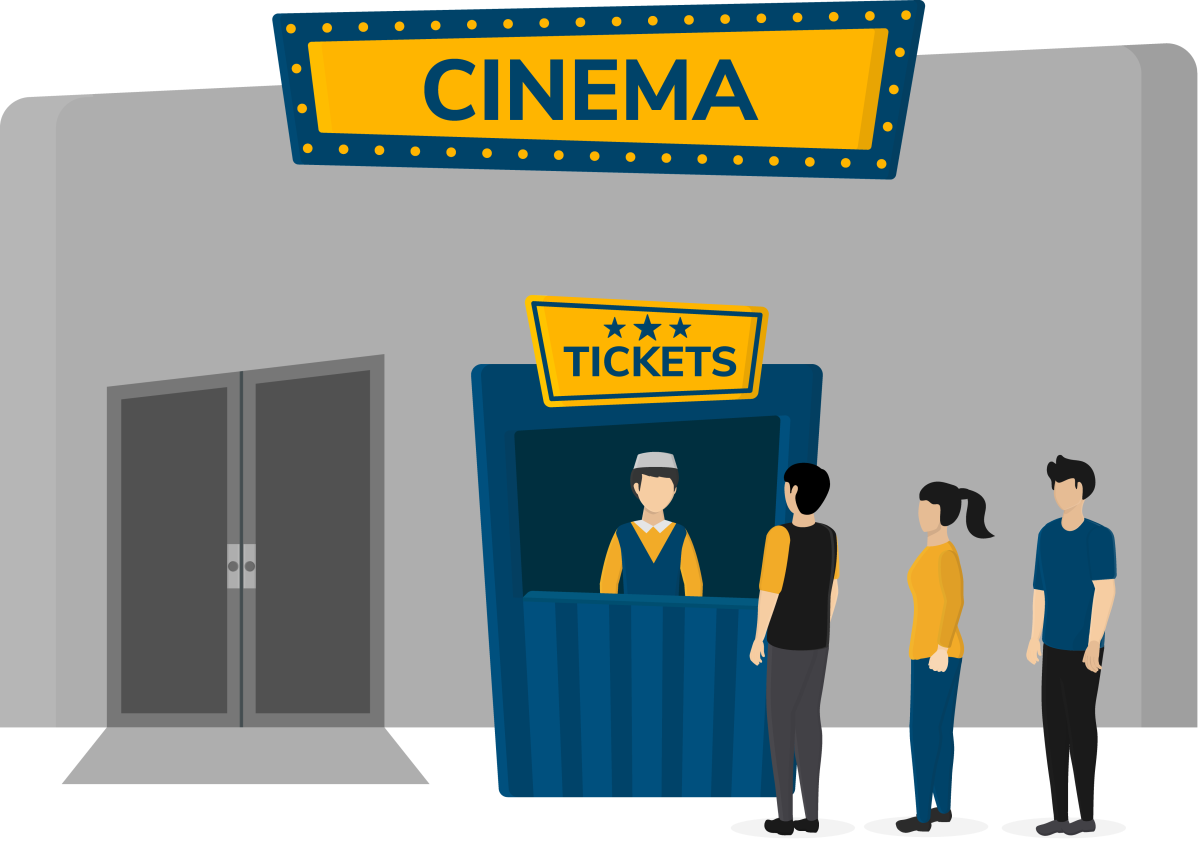
\includegraphics[width=0.15\textwidth]{Images/chapter_14/section_6553143930519552/5595744251936768.png}
 \caption{Customers are lining up to book tickets for a show}
\end{figure}

\subsection{Expectations from the interviewee}\label{DFpOXaHfjUJHQ4h6AROJx-2}
\\
A typical movie ticket booking system has numerous components, each with specific constraints and requirements. The following provides an overview of some of the main expectations that the interviewer will want to hear you discuss in more detail during the interview.

\subsubsection{Seat selection}\label{_e7rrB2ktLOwGTozRzsdM}
\\
Selecting a seat is an essential part of the movie ticket booking system. The system must ensure that no two people can book the same seat. The interviewer expects you to ask questions to identify how the system will work in these situations:

\begin{itemize}
\item
How will the system ensure multiple users do not book the same seat?
\item
Will there be a timeout session that temporarily reserves seats? Will the system use a first-come, first-served algorithm?
\item
Will there be transaction locks involved in the system?
\end{itemize}

\subsubsection{Payment handling}\label{eyHWHAHbyNYL3itm831JZ}
\\
One of the most significant attributes of the movie ticket booking system is the payment structure that it provides to its customers. This can vary, so the interviewer would expect you to ask the questions listed below:

\begin{itemize}
\item
\protect\phantomsection\label{WXru6qH9_qOo-vAqjjIcj}
What payment methods can the customer use (for example, credit card or cash)?
\item
\protect\phantomsection\label{gwf7hvnrKSzXhVIq0iiIS}
How is the payment performed? Does the customer pay themselves online or through a ticket agent at the location?
\end{itemize}

\subsubsection{Price variance}\label{ssGtkKIrSGy3NX5f_EtnS}
\\
We touched upon the payment methods of the movie ticket booking system. Now , the pricing model needs to be clarified by the interviewer, and therefore, you may ask questions like these:

\begin{itemize}
\item
\protect\phantomsection\label{Xv3Yng3O8bRBDkf4TVWaA}
How will the booking price be calculated? Will it vary based on the popularity of the show?
\item
\protect\phantomsection\label{S5_h4kViGjJvxk0LI8Jhu}
Does the seat type affect the pricing?
\item
\protect\phantomsection\label{nISofqLNYBxOhuvX9UcF7}
Will there be discount coupon codes?
\end{itemize}

\subsubsection{Duplication}\label{pJeX34_fRjJLE3liabeKv}
\\
There will be many duplicate instances in our system. The interviewer expects you to ask questions like these:

\begin{itemize}
\item
\protect\phantomsection\label{SgB6yqOqF8RYh1vMy7qdw}
How are we handling these instances, such as the same cinema having multiple cinema halls showing different movies simultaneously?
\item
\protect\phantomsection\label{yJJlAix0vbm2YFLyf0qkd}
Is the same movie shown in the same cinema/hall at different times?
\end{itemize}

\subsection{Design approach}\label{qYgIVqznecKd2pUDQYQ0b}
\\
We will design this movie ticket booking system using the bottom-up design approach. For this purpose, we will follow the steps below:

\begin{itemize}
\item
First, we'll identify core entities such as \texttt{Cinema}, \texttt{CinemaHall}, \texttt{Movie}, Show\ Seat, and \texttt{Booking}, and define their responsibilities.
\item
Next, we'll model how customers search for movies, view showtimes, and interact with seating layouts to reserve seats.
\item
We'll implement mechanisms to handle concurrency---preventing double bookings and managing seat reservations---while integrating reliable payment methods.
\end{itemize}
\\
This design approach will address edge cases (such as simultaneous seat selection), scalability, and SOLID principles for maintainable, extendable architecture. In later lessons, we'll illustrate major workflows with diagrams and code examples.

\subsection{Design pattern~}\label{MBdag8LJtJUJiiIih5k4L}
\\
Discussing the design patterns that a movie ticket booking system follows \hspace{0pt}\hspace{0pt} during an interview is always a good practice. Stating the design patterns gives the interviewer a positive impression and shows that the interviewee is well-versed in the advanced concepts of object-oriented design.
\\
Try to answer the following question. If you are not familiar with design patterns, don't worry! You can learn about them by asking, ``Define design patterns.''

\textbf{Question:}

Which design pattern(s) should be used to design a movie ticket booking system? Please elaborate on your choice(s).

Let's explore the requirements of the movie ticket booking system in the next lesson.

% End of section content